% !TeX program = lualatex
% !TeX encoding = utf8
% !TeX spellcheck = uk_UA
% !BIB program = bibler

\documentclass[9pt]{beamer}
\usetheme{Electromagnetism}
\usepackage{Electromagnetism}
\usepackage{physics}
\usepackage{tikz}
\usepackage{tikz-3dplot}
\usepackage[outline]{contour} % glow around text
\usepackage{xcolor}


\let\vect\vec
%============================================================================
\title[Лекції електрики та магнетизму]{\huge\bfseries Випромінювання електромагнітних хвиль}
\subtitle{Лекції з електрики та магнетизму}
\author{Пономаренко С. М.}
%============================================================================
\graphicspath{{pictures/}}
\begin{document}
\begin{frame}[plain]
	\maketitle
\end{frame}




% ============================== Слайд ## ===================================
\begin{frame}{Потенціали електромагнітного поля}{Калібрувальні перетворення}
	Задачу про випромінювання електромагнітних хвиль зручно розглядати за допомогою електромагнітних потенціалів $ \phi $ та $ \vect{A} $.
	\begin{align*}
		\divg\Bfield = 0                            & \Rightarrow \Bfield = \rot\vect{A},                                     \\
		\rot\Efield + \frac1c\parttime{\Bfield} = 0 & \Rightarrow \Efield = - \vect{\nabla}\phi - \frac1c\parttime{\vect{A}}.
	\end{align*}

	Потенціали визначаються не точно. Якщо змінити потенціали наступним чином:
	\begin{align*}
		\vect{A}' & = \vect{A} + \vect{\nabla} f,  \\
		\phi'     & = \phi - \frac1c \parttime{f},
	\end{align*}
	де $ f (x,y,z,t)$ --- довільна функція координат та часу, то спостережувані величини --- поля $ \Efield $ та $ \Bfield $ при таких перетвореннях не зміняться. Такі перетворення називаються \emph{калібрувальними перетвореннями}.
\end{frame}
% ===========================================================================




% ============================== Слайд ## ===================================
\begin{frame}{Потенціали електромагнітного поля}{Калібрування Лоренца}
	Запишемо рівняння Максвелла
	\begin{equation*}
		\rot\Bfield = \frac{4\pi\mu}{c}\vect{j} + \frac{\epsilon}{c}\parttime{\Efield}
	\end{equation*}
	через потенціали:
	\begin{equation*}
		\rot\rot\vect{A} = \frac{4\pi\mu}{c}\vect{j} + \frac{\epsilon\mu}{c} \parttime{}\left( - \vect{\nabla}\phi - \frac1c\parttime{\vect{A}}\right)
	\end{equation*}
	Використовуючи $ \rot\rot\vect{A} =   \vect{\nabla}(\divg\vect{A}) - \nabla^2\vect{A}$
	\begin{equation*}
		\nabla^2\vect{A} - \frac{ \epsilon\mu }{c^2} \pparttime{\vect{A}} = - \frac{4\pi\mu}{c}\vect{j} + \vect{\nabla}\left( \divg\vect{A} + \frac{\epsilon\mu}{c} \parttime\phi\right)
	\end{equation*}

	\begin{overprint}
		\onslide<1>
		Користуючись неоднозначністю потенціалів, визначених з
		точністю до калібрувального перетворення, можна на них накласти умову:
		\begin{equation*}
			\divg\vect{A} + \frac{\epsilon\mu}{c} \parttime\phi = 0.
		\end{equation*}
		Ця умова називається \emph{калібруванням Лоренца}.
		\onslide<2>
		Калібрування Лоренца аналогічне до вибору функції $ f $, такою, що задовольняє рівнянню
		\begin{equation*}
			\nabla^2 f - \frac{ \epsilon\mu }{c^2} \pparttime{f} = 0
		\end{equation*}
		{\scriptsize Рівняння є хвильовим рівнянням або однорідним рівнянням Даламбера.}
		\onslide<3>
		З урахуванням калібрування Лоренца отримуємо
		\begin{equation*}
			\nabla^2\vect{A} - \frac{ \epsilon\mu }{c^2} \pparttime{\vect{A}} = - \frac{4\pi\mu}{c}\vect{j}
		\end{equation*}
		{\scriptsize Рівняння є неоднорідним рівнянням Даламбера.}
	\end{overprint}
\end{frame}
% ===========================================================================




% ============================== Слайд ## ===================================
\begin{frame}{Рівняння для скалярного потенціалу}{}
	Використаємо рівняння Максвелла
	\begin{equation*}
		\divg\Efield = \frac{4\pi}{\epsilon} \rho
	\end{equation*}
	\begin{equation*}
		\divg \left( -\vect{\nabla}\phi - \frac1c\parttime{\vect{A}} \right) = \frac{4\pi}{\epsilon} \rho,
	\end{equation*}
	Використовуючи калібрування Лоренца
	\begin{equation*}
		\nabla^2\phi - \frac{ \epsilon\mu }{c^2} \pparttime{\phi} = - \frac{4\pi\rho}{\epsilon}
	\end{equation*}
\end{frame}
% ===========================================================================




% ============================== Слайд ## ===================================
\begin{frame}{Рівняння Даламбера для потенціалів}{}
	Отримали рівняння Даламбера для потенціалів:
	\begin{align*}
		\nabla^2\vect{A} - \frac{ \epsilon\mu }{c^2} \pparttime{\vect{A}} & = - \frac{4\pi\mu}{c}\vect{j}, \\
		\nabla^2\phi - \frac{ \epsilon\mu }{c^2} \pparttime{\phi}         & = - \frac{4\pi\rho}{\epsilon}.
	\end{align*}
	Розв'язками \emph{запізнюючі} потенціали:
	{\small 	\begin{equation*}
		\vect{A}(t)= \frac{\mu}{c} \iiint\limits_{V'} \frac{\vect{j}\left(\vect{r}', t - \frac{|\vect{r} - \vect{r}'|}{v}\right) dV'}{|\vect{r} - \vect{r}'|}, \quad
		\phi(t) = \frac{1}{\epsilon} \iiint\limits_{V'} \frac{\rho\left(\vect{r}', t - \frac{|\vect{r} - \vect{r}'|}{v}\right) dV'}{|\vect{r} - \vect{r}'|}
	\end{equation*}}

	\begin{overprint}
		\onslide<1>
		\begin{alertblock}{}\small\justifying
			В даний момент часу $ t $ в даній точці $ \vect{r} $ потенціал обумовлений не розподілом і величиною зарядів і струмів у даний момент часу, а їх положеннями та величинами у попередні моменти часу, що визначаються з урахуванням швидкості поширення електромагнітного поля.
		\end{alertblock}
		\onslide<2>
		\begin{alertblock}{}\small\justifying
			Потенціали називаються \emph{запізнюючими}, тому що вони описують потенціали в пізніший момент часу $ t $ в порівнянні з моментом часу $ t - \frac{|\vect{r} - \vect{r}'|}{v} $ для зарядів та струмів, які цей потенціал створили.
		\end{alertblock}
		\onslide<3>
		\begin{alertblock}{}\small\justifying
			Формально розв'язками рівнянь є також вирази в яких замінено знак <<$ - $>> на <<$ + $>> в аргументі. Розв'язки зі знаком <<$ + $>> в аргументі не мають ясного фізичного сенсу, оскільки вони формально відповідають ситуації, у якій спочатку створюється потенціал, а потім з'являються відповідні йому заряди та струми, тобто потенціал випереджає заряди та струми. Тому він називається \emph{випереджаючим}.
		\end{alertblock}
	\end{overprint}
\end{frame}
% ===========================================================================





% ============================== Слайд ## ===================================
\begin{frame}{Запізнюючі потенціали}{}
	{\small \begin{equation*}
			\vect{A}(t)= \frac{\mu}{c} \iiint\limits_{V'} \frac{\vect{j}\left(\vect{r}', t - \frac{|\vect{r} - \vect{r}'|}{v}\right) dV'}{|\vect{r} - \vect{r}'|}, \quad
			\phi(t) = \frac{1}{\epsilon} \iiint\limits_{V'} \frac{\rho\left(\vect{r}', t - \frac{|\vect{r} - \vect{r}'|}{v}\right) dV'}{|\vect{r} - \vect{r}'|}
		\end{equation*}}
	%---------------------------------------------------------
	\begin{center}
		\begin{tikzpicture}[scale=0.65, every node/.style={transform shape}]
			\pgfmathsetseed{90}
			\fill[gray!20] plot [smooth cycle, samples=8,domain={1:8}] (\x*360/8+6*rnd:1cm+2cm*rnd);
			\coordinate (O) at (0,0);
			\draw[-latex] (O) -- +(3,0) node[below] {$y$};
			\draw[-latex] (O) -- +(0,3) node[left] {$z$};
			\draw[-latex] (O) -- +(225:2.5) node[left] {$x$};
			\node[below] at (O) {$O$};

			\node[circle, fill=black, inner sep=0.025cm] (P) at (25:10) {};
			\node[right=10pt, font=\small, text width=2.5cm, align=center] at (P) {Поля в момент часу $ t $};
			\node[below] at (P) {$ P $};

			\node[ball color=gray!50, opacity=0.5, minimum size=0.1] (V) at (125:1.5) {};
			\node[above=10pt, opacity=1] at (V) {$dV'$};
			\draw[-latex] (O) --  node[pos=0.5, anchor=north east] {$\vect{r'}(t - \tau)$} (V);
			\draw[-latex] (O) -- node[pos=0.5, below] {$\vect{r}$} (P);
			\draw[-latex] (V) -- (P) node[pos=0.45, above, sloped] {$\vect{r} - \vect{r'}(t - \tau)$};

			\draw[decorate, decoration=snake, red, ultra thin] (V) -- (P);

		\end{tikzpicture}

		\begin{block}{}\justifying\small
			Поля у точці спостереження $ P $ в момент $ t $ залежать від того положення, яке заряди $ dV' $ займали у раніший момент часу $ t' = t - \frac{|\vect{r} - \vect{r}'|}{v} $. Де $ \tau =  \frac{|\vect{r} - \vect{r}'|}{v}$ --- час, необхідний. щоб збурення поля дійшло до точки $ P $.
		\end{block}
	\end{center}
	%---------------------------------------------------------
\end{frame}
% ===========================================================================





% ============================== Слайд ## ===================================
\begin{frame}{Математична довідка}
	Для випадку $ r \gg r' $, використовуючи формулу еквівалентності $ (1 + x)^n = 1 + nx $:
	\begin{equation*}
		|\vect{r} - \vect{r}'|  = \sqrt{r^2 -2\, \vect{r} \cdot \vect{r}' + r^{\prime 2} } \approx r - \frac{\vect{r} \cdot \vect{r}'}{r}.
	\end{equation*}

	\begin{equation*}
		\frac1{|\vect{r} - \vect{r}'|} \approx \frac1{r} + \frac{\vect{r} \cdot \vect{r}'}{r^3}.
	\end{equation*}

	\begin{equation*}
		t - \frac{|\vect{r} - \vect{r}'|}{c} \approx t - \frac{r}{c} + \frac{\vect{r} \cdot \vect{r}'}{cr} = \tau + \frac{\vect{r} \cdot \vect{r}'}{cr}.
	\end{equation*}
\end{frame}
% ===========================================================================





% ===========================================================================
\begin{frame}{Скалярний потенціал}{}
	\begin{onlyenv}<1>
		Далі покладемо $ \epsilon = \mu = 1 $.

		Розкладемо  в ряд Тейлора підінтегральну функцію  по степеням малої величини $  \frac{\vect{r} \cdot \vect{r}'}{cr} $
		\begin{multline*}
			\phi(t) = \iiint\limits_{V'}\frac{\rho\left(\vect{r}', t - \frac{|\vect{r} - \vect{r}'|}{c}\right)  dV'}{|\vect{r} - \vect{r}'|} \approx \\ \approx
			\iiint\limits_{V'} \left( \rho(\tau) +  \frac{\vect{r} \vect{r}'}{cr} \dot{\rho}(\tau)\right) \left[ \frac1{r} + \frac{\vect{r}  \vect{r}'}{r^3} \right]dV' \approx \\
			\approx \frac1r\iiint\limits_{V'} {\rho(\tau)} dV' + \frac{\vect{r}  }{r^3}\iiint\limits_{V'}\rho(\tau)\vect{r}' dV' + \frac{\vect{r} }{cr^2}\iiint\limits_{V'} \dot{\rho}(\tau) \vect{r}'dV' = \\
			= \frac{q}{r} + \frac{\vect{r}\vect{p}}{r^3} + \frac{\vect{r}\dot{\vect{p}}}{cr^2}.
		\end{multline*}
	\end{onlyenv}
	\begin{onlyenv}<2>
		Для електронейтральних тіл $ q = 0 $, тому
		\begin{equation*}
			\phi(t)  = \frac{\vect{r}\vect{p}}{r^3} + \frac{\vect{r}\dot{\vect{p}}}{cr^2}.
		\end{equation*}

		Спростимо останній вираз, помітивши, що

		\begin{equation*}
			-\divg\frac{\vect{p}}{r} = -\vect{p}\overbrace{\cdot\vect{\nabla}\frac1r}^{-\frac{\vect{r}}{r^3}} - \frac1r\overbrace{\divg\vect{p}}^{-\frac{\dot{\vect{p}}\vect{r}}{cr}}.
		\end{equation*}

		\begin{equation*}
			\divg\vect{p} = \frac{\partial p_x}{\partial x} + \frac{\partial p_y}{\partial y} + \frac{\partial p_z}{\partial z} = \frac{\partial p_x}{\partial \tau}\frac{\partial\tau}{\partial x} + \frac{\partial p_y}{\partial \tau}\frac{\partial\tau}{\partial y} +\frac{\partial p_z}{\partial \tau}\frac{\partial\tau}{\partial z} = -\frac{\dot{\vect{p}}\vect{r}}{cr}.
		\end{equation*}

		Отже,
		\begin{equation*}
			\phi(t) = -\divg\left( \frac{\vect{p}\left(t - \frac{r}{c}\right)}{r} \right).
		\end{equation*}
	\end{onlyenv}
\end{frame}
% ===========================================================================




% ============================== Слайд ## ===================================
\begin{frame}{Векторний потенціал}{}
	\begin{onlyenv}<1>
		\begin{multline*}
			\vect{A}(t) = \frac1c\iiint\limits_{V'}\frac{\vect{j}\left(\vect{r}', t - \frac{|\vect{r} - \vect{r}'|}{c}\right)  dV'}{|\vect{r} - \vect{r}'|} \approx \\ \approx
			\frac1c\iiint\limits_{V'} \left( \vect{j}(\tau) +  \frac{\vect{r} \vect{r}'}{cr} \dot{\vect{j}}(\tau)\right) \left[ \frac1{r} + \frac{\vect{r}  \vect{r}'}{r^3} \right]dV' \approx \\
			\approx \frac1{cr}\iiint\limits_{V'} {\vect{j}(\tau)} dV'
		\end{multline*}

		\begin{block}{}\justifying
			Ми можемо обмежилися лише першим членом цього розкладання. Як показують розрахунки, наступні доданки пов'язані з магніто-дипольною складовою випромінювання.
		\end{block}
	\end{onlyenv}
	\begin{onlyenv}<2>
		\begin{equation*}
			\vect{A}(t) \approx \frac1{cr}\iiint\limits_{V'} {\vect{j}(\tau)} dV'
		\end{equation*}

		Закон збереження заряду
		\begin{equation*}
			\parttime{\rho(x',y',z', t)} = -\vect{\nabla}'\vect{j}(x',y',z', t),
		\end{equation*}
		де $ \vect{\nabla}' $ означає диференціювання по координатам $ x' $, $ y' $, $ z' $.
		\begin{equation*}
			\parttime{}\vect{p}(\tau) = -\iiint\limits_{V'}\vect{r}'\vect{\nabla}'\cdot\vect{j}(x',y',z', t) dV',
		\end{equation*}
		Використаємо співвідношення:
		\begin{equation*}
			(\vect{a}\vect{r}')\vect{\nabla}'\cdot\vect{j} =  \vect{\nabla}'\cdot(\vect{j(\vect{a}\vect{r}')}) - \vect{j}\vect{\nabla}'(\vect{a}\vect{r}') = \vect{\nabla}'\cdot(\vect{j(\vect{a}\vect{r}')}) - \vect{a}\vect{j}.
		\end{equation*}
		де $ \vect{a} $ ($ a = 1 $) довільний постійний вектор.
	\end{onlyenv}
	\begin{onlyenv}<3>
		\begin{equation*}
			\vect{a} \parttime{}\vect{p}(\tau) = -\iiint\limits_{V'}\vect{\nabla}'\cdot(\vect{j(\vect{a}\vect{r}')}) dV' + \vect{a} \iiint\limits_{V'} {\vect{j}(\tau)} dV',
		\end{equation*}
		\begin{block}{}\justifying
			Перший інтеграл може бути за допомогою теореми Гауса перетворений в інтеграл поверхні $ S' $, що охоплює об'єм $ V' $. Оскільки всі електричні заряди, за умовою, перебувають усередині обсягу об'ємі $ V' $, через граничну поверхню $ S' $ струмів не протікає, тобто на ній $ \vect{j} = 0 $  і, отже, дорівнює нулю.
		\end{block}

		\medskip

		Отримали
		\begin{equation*}
			\parttime{}\vect{p}(\tau) = \iiint\limits_{V'} {\vect{j}(\tau)} dV',
		\end{equation*}

		Отже
		\begin{equation*}
			\vect{A}(t) \approx \frac1{c}\parttime{}\left( \frac{\vect{p}\left(t - \frac{r}{c}\right)}{r} \right)
		\end{equation*}
	\end{onlyenv}

\end{frame}
% ===========================================================================




% ============================== Слайд ## ===================================
\begin{frame}{Зауваження після виведення}{}\scriptsize
	\begin{block}{}
		В формулі
		\begin{equation*}
			t' =  t - \frac{r}{c} + \frac{\vect{r} \cdot \vect{r}'}{cr}
		\end{equation*}
		час $ \frac{\vect{r}\vect{r}'}{cr} $ --- є часом власним часом запізнення елемента $ dV' $ (запізнення по відношенню до вибраного <<центру>> системи) і при виведенні всіх формул є  його вважали малим в порівняння часом загального запізнення $ \frac{r}{c} $.
	\end{block}

	\begin{block}{}\justifying
		Крім цього, необхідно, щоб за час власного запізнення не надто сильно змінювалися густини зарядів $ \rho $ і струмів $ \vect{j} $, інакше не можна буде користуватися розкладами через великі значення похідних за часом $ \dot\rho $ і струмів $ \dot{\vect{j}} $. Заряди в системі за час власного запізнення проходять відстань порядку $ \frac{vr'}{c} $. Якщо ця відстань мала порівняно з розмірами системи $ r' $, то за час власного запізнення розташування зарядів суттєво не змінюється і прийняте наближення допустиме.
	\end{block}

	\begin{block}{}
		Умовою його застосування служить сильна нерівність $ v\frac{r'}{c} \ll r' $ з якої випливає
		\begin{equation*}
			v \ll c,
		\end{equation*}
		тобто, швидкості руху зарядів у системі повинні бути нерелятивістськими.
	\end{block}
\end{frame}
% ===========================================================================





% ============================== Слайд ## ===================================
\begin{frame}{Елементарний дипольний випромінювач}{}
	\begin{alertblock}{}\centering
		Монопольного випромінювання не існує!
	\end{alertblock}

	Розглянемо електронейтральну систему --- електричний диполь, який є елементарним вимпромінювачем електромагнітних хвиль.
	\begin{center}
		\begin{tikzpicture}
			\draw[thick, red, double, -stealth] (0,-0.5) node[right, font=\scriptsize] {диполь в момент часу $ t' =  t - \frac{r}{c} $} -- ++(0,1) node[left] {$\vect{p}_0$};
			\draw[-latex] (0,0) -- node[anchor=south east] {$\vect{r}$} node[below, sloped] {$ \Delta t = r/c $} (25:4) node[right, font=\scriptsize] {Поля в момент часу $ t $};
		\end{tikzpicture}
	\end{center}

	Дипольний момент $ \vect{p} $ змінюється за гармонічним законом:
	\begin{equation*}
		\vect{p} = \vect{p}_0 \cos\omega t, \quad 	\vect{p} = \vect{p}_0e^{i\omega t}\, \text{(в комплексній формі)}
	\end{equation*}

	\begin{block}{}
		Крім елементарного дипольного випромінювача ще існують елементарний магніто-дипольний випромінювач, квадрупольний \ldots
	\end{block}
\end{frame}
% ===========================================================================




% ============================== Слайд ## ===================================
\begin{frame}{Запізнюючі потенціали для диполя}{}
	\begin{align*}
		\vect{A}(t) & = \frac1c \parttime{}\left( \frac{\vect{p}\left(t - \frac{r}{c}\right)}{r} \right)  = \frac1c \parttime{\vect{P}(t)},                \\
		\phi(t)     & = -\frac{\vect{r}}{r} \frac{\partial}{\partial r}\left( \frac{\vect{p}\left(t - \frac{r}{c}\right)}{r} \right) =  -\divg\vect{P}(t),
	\end{align*}
	де $ \vect{P}(t) $ --- вектор Герца:
	\begin{equation*}
		\vect{P}(t) = \frac{\vect{p}\left(t - \frac{r}{c}\right)}{r}, \quad \nabla^2\vect{P} - \frac{1}{c^2}\pparttime{\vect{P}} = 0
	\end{equation*}
	$ \vect{p} $ --- дипольний момент.

	\begin{block}{}\small\justifying
		Як випливає з цього рівняння, значення вектора Герца в
		момент $ t $ у точці, що знаходиться на відстані $ r $ від осцилятора,
		визначається значенням дипольного моменту осцилятора
		момент $ t - r / c $.
	\end{block}{}
\end{frame}
% ===========================================================================





% ============================== Слайд ## ===================================
\begin{frame}{Поля диполя}{}
	\begin{equation*}
		\Bfield = \rot\vect{A} = \frac1c \parttime{} \rot\vect{P}, \quad
		\Efield = - \vect{\nabla}\phi - \frac1c\parttime{\vect{A}} = \rot\rot\vect{P}.
	\end{equation*}
	\begin{alertblock}{}
		Таким чином, задача визначення $ \Bfield $ і $ \Efield $ зведено до обчислення ротора вектора $ \vect{P} $ та його похідних.
	\end{alertblock}
	\begin{block}{}\small
		Якщо момент диполя змінюється за гармонічним законом $ \vect{p} = \vect{p}_0 e^{ш\omega t} $, то вектор герца змінюватиметься за законом
		$ \vect{P} = \frac{\vect{p}_0 e^{i\omega (t - r/c)}}{r} $, а поля змінюватимуться за законами (в сферичних координатах):
	\end{block}
	%---------------------------------------------------------
	\begin{minipage}{0.7\linewidth}\centering
		\begin{align*}\small
			B_{\phi}   & = \frac{i\omega}{c}\sin\theta\left( \frac1r + \frac{i\omega}{c}\right) P,                \\
			E_r        & = 2\cos\theta\left( \frac{1}{r^2} + \frac{i\omega}{cr}\right) P,                         \\
			E_{\theta} & = \sin\theta \left( \frac{1}{r^2} + \frac{i\omega}{cr} - \frac{\omega^2}{c^2} \right) P.
		\end{align*}
	\end{minipage}%
	%---------------------------------------------------------
	\begin{minipage}{0.3\linewidth}\centering
		\tdplotsetmaincoords{60}{110}
		%
		\pgfmathsetmacro{\rvec}{.8}
		\pgfmathsetmacro{\thetavec}{30}
		\pgfmathsetmacro{\phivec}{60}
		%
		\begin{tikzpicture}[scale=2,tdplot_main_coords, >=latex]
			\coordinate (O) at (0,0,0);
			\draw[thick,->] (0,0,0) -- (1,0,0) node[anchor=north east]{$x$};
			\draw[thick,->] (0,0,0) -- (0,1,0) node[anchor=north west]{$y$};
			\draw[thick,->] (0,0,0) -- (0,0,1) node[anchor=south]{$z$};
			\tdplotsetcoord{P}{\rvec}{\thetavec}{\phivec}
			\draw[-stealth, green!50!black] (O) -- (P);
			\draw[dashed, color=red] (O) -- (Pxy);
			\draw[dashed, color=red] (P) -- (Pxy);
			\tdplotdrawarc{(O)}{0.2}{0}{\phivec}{anchor=north}{$\phi$}
			\tdplotsetthetaplanecoords{\phivec}
			\tdplotdrawarc[tdplot_rotated_coords]{(0,0,0)}{0.5}{0}%
			{\thetavec}{anchor=south}{$\theta$}
			\draw[dashed,tdplot_rotated_coords] (\rvec,0,0) arc (0:90:\rvec);
			\draw[dashed] (\rvec,0,0) arc (0:90:\rvec);
			\tdplotsetrotatedcoords{\phivec}{\thetavec}{0}
			\tdplotsetrotatedcoordsorigin{(P)}
			\draw[thick,tdplot_rotated_coords,->, red] (0,0,0)
			-- (.25,0,0) node[anchor=north west]{$\vec{e}_{\theta}$};
			\draw[thick,tdplot_rotated_coords,->,blue] (0,0,0)
			-- (0,.25,0) node[anchor=west]{$\vec{e}_{\phi}$};
			\draw[thick,tdplot_rotated_coords,->, green!50!black] (0,0,0)
			-- (0,0,.25) node[anchor=south]{$\vec{e}_{r}$};
		\end{tikzpicture}
	\end{minipage}
	%---------------------------------------------------------
\end{frame}
% ===========================================================================




% ============================== Слайд ## ===================================
\begin{frame}{Поля диполя}{Ближня зона}
	\begin{block}{}
		Ближня зона --- відстань від осцилятора до точки спостереження  мала в порівнянні з
		довжиною його хвилі:
		\begin{equation*}
			\frac1r \gg \frac{\omega}c, \quad	r \ll \frac{\lambda}{2\pi}
		\end{equation*}
	\end{block}

	\begin{overprint}
		\onslide<1>
		\begin{block}{}
			В кожен момент часу $ t $ електричне поле поблизу
			зі осцилятора збігається з полем статичного диполя, дипольний момент якого дорівнює миттєвого значення моменту осцилятора $  p(t) $:
			\begin{align*}
				E_r        & = \frac{2\cos\theta p(t)}{r^3},  \\
				E_{\theta} & =  \frac{\sin\theta p(t)}{r^3} .
			\end{align*}
		\end{block}
		\onslide<2>
		\begin{block}{}
			Оскільки
			\begin{equation*}
				\parttime{p(t)} = \parttime{q(t)l} = \parttime{q(t)}l = I l,
			\end{equation*}
			магнітне поле збігається з полем еквівалентного елемента струму довжини $ l $, що визначається формулою Біо-Савара-Лаплпса:
			\begin{equation*}
				\Bfield   = \frac{1}{cr^3} \left[ \parttime{\vect{p}(t)}\times\vect{r}\right] = \frac{I}{c} \frac{\left[ \vect{l}\times\vect{r}\right] }{r^3},
			\end{equation*}
		\end{block}
		\onslide<3>
		\begin{alertblock}{}
			В ближній зоні поля не запізнюються і співпадають з полями статичного диполя та струму.
		\end{alertblock}
	\end{overprint}
\end{frame}
% ===========================================================================





% ============================== Слайд ## ===================================
\begin{frame}{Поля диполя}{Хвильова зона}
	\begin{block}{}
		Відстань, яка набагато більша за довжину хвилі:
		\begin{equation*}
			\frac1r \ll \frac{\omega}c, \quad r \gg \frac{\lambda}{2\pi}
		\end{equation*}
		називається \emph{хвильовою зоною}.
	\end{block}
	\vspace*{-1em}
	\begin{columns}
		\begin{column}{0.7\linewidth}
			\begin{align*}
				E_{\theta} & = B_{\phi} = -\frac{\omega^2\sin\theta}{c^2 r}p_0\cos\omega\left(t - \frac{r}{c} \right) = \\
				           & = \frac{\sin\theta}{rc^2}  \ddot{p}\left(t - \frac{r}{c}\right),                           \\
				E_r        & = E_{\phi} = B_r = B_{\theta} = 0 .
			\end{align*}
		\end{column}
		\begin{column}{0.3\linewidth}
			\begin{overprint}
				\onslide<1>
				\begin{center}
					\tdplotsetmaincoords{60}{110}
					%
					\pgfmathsetmacro{\rvec}{.8}
					\pgfmathsetmacro{\thetavec}{30}
					\pgfmathsetmacro{\phivec}{60}
					%
					\begin{tikzpicture}[scale=2.2,tdplot_main_coords, >=latex]
						\coordinate (O) at (0,0,0);
						\draw[thick,->] (0,0,0) -- (1,0,0) node[anchor=north east]{$x$};
						\draw[thick,->] (0,0,0) -- (0,1,0) node[anchor=north west]{$y$};
						\draw[thick,->] (0,0,0) -- (0,0,1) node[anchor=south]{$z$};

						\tdplotsetcoord{P}{\rvec}{\thetavec}{\phivec}
						\draw[-stealth, green!50!black] (O) -- (P);
						\draw[ultra thick, -stealth, red] (0,0,-0.15) -- (0,0,0.15) node[anchor=east]{$\vec{p}_0$};
						\draw[dashed, color=red] (O) -- (Pxy);
						\draw[dashed, color=red] (P) -- (Pxy);
						\tdplotdrawarc{(O)}{0.2}{0}{\phivec}{anchor=north}{$\phi$}
						\tdplotsetthetaplanecoords{\phivec}
						\tdplotdrawarc[tdplot_rotated_coords]{(0,0,0)}{0.5}{0}%
						{\thetavec}{anchor=south}{$\theta$}
						\draw[dashed,tdplot_rotated_coords] (\rvec,0,0) arc (0:90:\rvec);
						\draw[dashed] (\rvec,0,0) arc (0:90:\rvec);
						\tdplotsetrotatedcoords{\phivec}{\thetavec}{0}
						\tdplotsetrotatedcoordsorigin{(P)}
						\draw[thick,tdplot_rotated_coords,->, red] (0,0,0)
						-- (.25,0,0) node[anchor=north west, inner sep=0]{${E}_{\theta}$};
						\draw[thick,tdplot_rotated_coords,->,blue] (0,0,0)
						-- (0,.25,0) node[anchor=west, inner sep=0]{${B}_{\phi}$};
						%                \draw[thick,tdplot_rotated_coords,->, green!50!black] (0,0,0)
						%                -- (0,0,.25) node[anchor=south]{$\vec{e}_{r}$};
					\end{tikzpicture}
				\end{center}
				\onslide<2>
				\begin{center}
					\begin{tikzpicture}[>=stealth]
						\draw[thick,color=blue,domain=0:2*pi,samples=200,smooth, name path=leaf] plot (xy polar cs:angle=\x r,radius= {1.5*abs(cos(\x r))});
						\draw[->, red, ultra thick] (0,-1) -- (0,1) node[left] {$ \vec{p} $};

                        \def\a{20}
						\draw (0,0) ++ (0,0.5) arc[start angle=90, end angle=\a, radius=0.5] node[pos=0.6, anchor=south west] {$ \theta $};
						\draw[name path=rule] (0,0) -- (\a:2);


						\node[text width=2cm, font=\tiny, align=center, inner sep=0, gray] (TEXT) at (0.5,-1.6) {Довжина відрізка\\ дорівнює\\ величині поля};

						\path[name intersections={of=leaf and rule}] (intersection-1) coordinate (E);

						\draw[->, gray] (TEXT.100) to[out=90, in=-15] (0,0);
						\draw[->, gray] (TEXT.80) to[out=90, in=270] (E);
					\end{tikzpicture}
				\end{center}
			\end{overprint}
		\end{column}
	\end{columns}
	\begin{overprint}
		\onslide<1>
		\begin{alertblock}{}\scriptsize\justifying
			У хвильовій зоні осцилятора електричне та магнітне полія чисельно дорівнюють один одному і спадають обернено пропорційно першій степені відстані від осцилятора.
		\end{alertblock}
		\onslide<2>
		\begin{alertblock}{}\scriptsize\justifying
			Напруженість поля також залежить від полярного
			кута $\theta$ точки спостереження: на продовженні осі осцилятора ($ \theta = 0 $ і $ \theta = \pi $) поле дорівнює нулю, максимального ж
			значення воно досягає в екваторіальній площині осцилятора ($ \theta = \pi/2 $). У кожній точці хвильової зони вектори $ \Efield $, $ \Bfield $ та $ \vect{r} $ взаємно перпендикулярні та утворюють правогвинтову систему.
		\end{alertblock}
	\end{overprint}

\end{frame}
% ===========================================================================





% ============================== Слайд ## ===================================
\begin{frame}{Ближня та хвильова зони}{}
	\begin{center}
		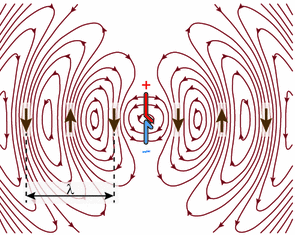
\includegraphics[width=0.5\linewidth]{dipole_radiation}
	\end{center}
	\begin{block}{}\justifying
		В ближній зоні поле ніби <<причеплене>> до диполя, а у хвильовій зоні поле <<відривається>> від нього --- випромінюється.
	\end{block}

	\vfill

	{\tiny \url{https://youtu.be/NPJinVFqC1s}}
\end{frame}
% ===========================================================================




% ============================== Слайд ## ===================================
\begin{frame}{Потужність, що випромінюється осцилятором}{}
	\begin{block}{}\justifying\small
		Густина потоку електромагнітної енергії характеризується вектором Пойнтінга $ \vect{S} $. Тому потік електромагнітної, енергії крізь поверхню сфери радіусом $ r $, що оточує осцилятор, називається \emph{потужністю випромінювання}.
	\end{block}
	\vspace*{-1em}
	\begin{overprint}
		\onslide<1>
		\begin{columns}
			\begin{column}{0.5\linewidth}
				\begin{center}
					\colorlet{veccol}{green!50!black}
					\colorlet{projcol}{black}
					\colorlet{myblue}{blue!80!black}
					\colorlet{myred}{red!90!black}
					\colorlet{mydarkblue}{blue!50!black}
					\tikzset{>=latex} % for LaTeX arrow head
					\tikzstyle{proj}=[projcol!80,line width=0.08] %very thin
					\tikzstyle{area}=[draw=veccol,fill=veccol!80,fill opacity=0.6]
					\tikzstyle{vector}=[-stealth,myblue,thick,line cap=round]
					\tikzstyle{unit vector}=[->,veccol,thick,line cap=round]
					\tikzstyle{dark unit vector}=[unit vector,veccol!70!black]
					\usetikzlibrary{angles,quotes} % for pic (angle labels)
					\contourlength{1.3pt}
					% 3D AXIS with spherical coordinates, dA
					\tdplotsetmaincoords{60}{103}
					\begin{tikzpicture}[scale=3,tdplot_main_coords, every node/.style={font=\scriptsize}]

						% VARIABLE
						\def\rvec{1.0}
						\def\thetavec{35}
						\def\phivec{45}
						\def\dtheta{10}
						\def\dphi{16}
						%  \def\sphere#1#2#3{plot[domain=#1]({\rvec*sin(#2)*cos(#3)},{\rvec*sin(#2)*sin(#3)},{\rvec*cos(#2)})}
						\contourlength{0.8pt}

						% AXES
						\coordinate (O) at (0,0,0);

						\draw[thick,->] (0,0,0) -- (1.16*\rvec,0,0) node[left,below]{$x$};
						\draw[thick,->] (0,0,0) -- (0,1.1*\rvec,0) node[below,right=0]{$y$};
						\draw[thick,->] (0,0,0) -- (0,0,1.1*\rvec) node[above]{$z$};

   						\draw[ultra thick, -latex, red] (0,0,-0.1) -- (0,0,0.1) node[left] {$ \vect{p}_0 $};

						% COORDINATES
						\tdplotsetcoord{P}{\rvec}{\thetavec}{\phivec}
						\tdplotsetcoord{PB}{\rvec}{\thetavec+\dtheta}{\phivec}
						\tdplotsetcoord{PR}{\rvec}{\thetavec}{\phivec+\dphi}
						\tdplotsetcoord{PBR}{\rvec}{\thetavec+\dtheta}{\phivec+\dphi}


						% CONE
						\draw[veccol!20,very thin] (O)  -- (PBR);
						\draw[veccol!20,very thin] (O)  -- (PR);
						\draw[->,veccol] (O)  -- (P) node[below,left, text=black] {$\vect{r}$};
						\draw[veccol,very thin] (O)  -- (PB);

						% PROJECTIONS
						\draw[proj] %\thetavec+\dtheta
						plot[domain=0:90]({\rvec*sin(\x)*cos(\phivec)},{\rvec*sin(\x)*sin(\phivec)},{\rvec*cos(\x)}) coordinate (BL);
						\draw[proj]
						plot[domain=0:90]({\rvec*sin(\x)*cos(\phivec+\dphi)},{\rvec*sin(\x)*sin(\phivec+\dphi)},{\rvec*cos(\x)}) coordinate (BR);
						\draw[proj]
						plot[domain=0:90]({\rvec*cos(\x)},{\rvec*sin(\x)},0);
						\draw[proj] (O)  -- (BL); % PBxy
						\draw[proj] (O)  -- (BR); % PBRxy
						\draw[proj] (P)  -- (Pz);
						\draw[gray] (PR)  -- (Pz) node[midway,above,rotate=-24] {\contour{white}{$r\sin\theta$}};
						%\draw[proj,projcol!15,dashed] (P) -- (Pxy);
						%\draw[proj,projcol!15,dashed] (PR) -- (PRxy);
						%\draw[proj,projcol!15,dashed] (PB) -- (PBxy);
						%\draw[proj,projcol!15,dashed] (PBR) -- (PBRxy);

						% AREA
						\draw[area]
						plot[domain=0:.99*\dphi]({\rvec*sin(\thetavec)*cos(\phivec+\x)},{\rvec*sin(\thetavec)*sin(\phivec+\x)},{\rvec*cos(\thetavec)}) --
						plot[domain=0:.99*\dtheta]({\rvec*sin(\thetavec+\x)*cos(\phivec+\dphi)},{\rvec*sin(\thetavec+\x)*sin(\phivec+\dphi)},{\rvec*cos(\thetavec+\x)}) --
						plot[domain=.99*\dphi:0]({\rvec*sin(\thetavec+\dtheta)*cos(\phivec+\x)},{\rvec*sin(\thetavec+\dtheta)*sin(\phivec+\x)},{\rvec*cos(\thetavec+\dtheta)}) --
						plot[domain=.99*\dtheta:0]({\rvec*sin(\thetavec+\x)*cos(\phivec)},{\rvec*sin(\thetavec+\x)*sin(\phivec)},{\rvec*cos(\thetavec+\x)}) --
						cycle;

						% MEASURES
						%\node[right=3,below right=-2] at (PB) {$r\sin\theta\dd{\phi}$};
						%\node[right=5,below right=-2] at (PR) {$r\dd{\theta}$};
						\draw[<->,gray,thin]
						plot[domain=0:\dphi]({\rvec*sin(\thetavec+1.11*\dtheta)*cos(\phivec+\x)},{\rvec*sin(\thetavec+1.11*\dtheta)*sin(\phivec+\x)},{\rvec*cos(\thetavec+1.11*\dtheta)})
						node[right=0.6,below] {\contour{white}{$r\sin\theta\dd{\phi}$}};
						\draw[<->,gray,thin]
						plot[domain=0:\dtheta]({\rvec*sin(\thetavec+\x)*cos(\phivec+1.15*\dphi)},{\rvec*sin(\thetavec+\x)*sin(\phivec+1.15*\dphi)},{\rvec*cos(\thetavec+\x)})
						node[above=-0.2,right] {$r\dd{\theta}$};

						% ANGLES
						\tdplotdrawarc[->]{(O)}{0.35*\rvec}{0}{\phivec}
						{below}{$\phi$}
						\tdplotdrawarc[->]{(O)}{0.45*\rvec}{\phivec}{\phivec+\dphi}
						{anchor=145,inner sep=1}{\contour{white}{$\dd{\phi}$}}
						\tdplotsetthetaplanecoords{\phivec}
						\tdplotdrawarc[->,tdplot_rotated_coords]{(0,0,0)}{0.36*\rvec}{0}{\thetavec}
						{right,above}{$\theta$}
						\tdplotdrawarc[->,tdplot_rotated_coords]{(0,0,0)}{0.54*\rvec}{\thetavec}{\thetavec+\dtheta}
						{left=0.2,above right}{\contour{white}{$\dd{\theta}$}}

                        % rotated coords
  						\tdplotsetcoord{F}{1}{40}{53}
                        \tdplotsetrotatedcoords{\phivec}{\thetavec}{0}
						\tdplotsetrotatedcoordsorigin{(F)}

  						\draw[tdplot_rotated_coords, ->] (0,0,0) -- (0,0,0.75) node[above, inner sep=0] {$ \vect{S} $};
  						\draw[tdplot_rotated_coords, ->, red] (0,0,0) -- (0.25,0,0) node[below, inner sep=0] {$ \Efield $};
  						\draw[tdplot_rotated_coords, ->, blue] (0,0,0) -- (0,0.25,0) node[anchor=south west, inner sep=0] {$ \Bfield $};
  						\draw[tdplot_rotated_coords, ->, green!50!black] (0,0,0) -- (0,0,0.4) node[anchor=south east, inner sep=1pt] {$ \vect{n} $};

					\end{tikzpicture}
				\end{center}
			\end{column}
			\begin{column}{0.5\linewidth}
				Елемент площі поверхні в сферичній системі координат
				\begin{equation*}
					d\sigma = r^2\sin\theta d\theta d\phi
				\end{equation*}

				\medskip

				Вектор орієнтованої площадки
				\begin{equation*}
					d\vect{\sigma} = d\sigma \vect{n} .
				\end{equation*}

				\medskip

				Як видно з рисунку $ \vect{S}\uparrow\uparrow\vect{n} $.
			\end{column}
		\end{columns}

		\onslide<2>
		\begin{multline*}
			\frac{dW}{dt} = -\oiint\limits_{\sigma} \vect{S}d \vect{\sigma} =  -\int\limits_0^{2\pi}\int\limits_0^{\pi} \frac{c}{4\pi}|[\Efield\times\Bfield]| \, r^2\sin\theta d\theta d\phi = \\
			=  \frac{\ddot{p}^2 \left( t - \frac{r}{c}\right) }{4\pi c^3} \int\limits_0^{\pi} \sin^3\theta d\theta \int\limits_0^{2\pi} d\phi = \frac{2\ddot{p}^2 \left( t - \frac{r}{c}\right) }{3c^3}
		\end{multline*}

		Середнє значення потужності випромінювання за період:
		\begin{equation*}
			\left\langle \frac{d W}{dt} \right\rangle = \frac1T\int\limits_0^T \frac{dW}{dt} dt = \frac{\omega^4p_0^2}{3c^3}
		\end{equation*}
		\onslide<3>
		\begin{block}{}\scriptsize\justifying
			Таким чином, осцилятор неперервно випромінює енергію в навколишній простір, причому, середня швидкість випромінювання енергії
			\begin{equation*}
				\left\langle \frac{d W}{dt} \right\rangle = \frac1T\int\limits_0^T \frac{dW}{dt} dt = \frac{\omega^4p_0^2}{3c^3}
			\end{equation*}
			пропорційна квадрату амплітуди його електричного моменту $ p_0 $ і пропорційна четвертій степені частоти $ \omega $.

			\medskip


			Цією останньою обставиною пояснюється, наприклад, той факт, що для радіозв'язку необхідно користуватися порівняно короткими електромагнітними хвилями довжиною від десятків метрів до десятків кілометрів; навпаки, випромінювання повільно змінних струмів, що застосовуються в техніці (хвилі довжиною в тисячі та десятки тисяч кілометрів), залишається практично непомітним.

		\end{block}
		\onslide<4>
        \vspace*{1em}
        \begin{tcolorbox}[enhanced,title={Колір неба},watermark graphics=BlueSky,
        watermark opacity=0.5,watermark color=blue,watermark stretch=1]
        \scriptsize\justifying
			Тим же характером залежності випромінювання осцилятора від
			частоти пояснюється, наприклад, блакитний колір неба. Сонячне світло, що пронизує атмосферу, розсіюється молекулами повітря, які можна вважати елементарним осциляторами. Розсіювання світла обумовлюється тим, що під впливом світлових хвиль ці осцилятори здійснюють <<вимушені>>
			коливання. Так як період власних коливань осциляторів, відповідних молекул повітря, істотно відрізняється від періоду видимого світла (відсутність резонансу), то амплітуда вимушених коливань осциляторів слабо залежить від частоти (або довжини) світлової хвилі. Тому інтенсивність
			розсіяного світла, тобто інтенсивність вимушеного випромінювання
			цих осциляторів, обернено пропорційна $ \lambda^4 $. Таким чином, короткохвильове світло (синій колір) розсіюється сильніше, ніж,
			наприклад, червоний, і створює блакитний колір неба.
		\end{tcolorbox}
	\end{overprint}
\end{frame}
% ===========================================================================





% ============================== Слайд ## ===================================
\begin{frame}{Випромінювання рухомого заряду}{}
	\begin{overprint}
		\onslide<1>
		\begin{block}{}\justifying
			Припустимо, що диполь складається з двох точкових зарядів: $ +q $ і $ -q $, з яких додатній нескінченно важкий, а тому його можна вважати нерухомим.
		\end{block}
		\onslide<2>
		\begin{block}{}\centering
			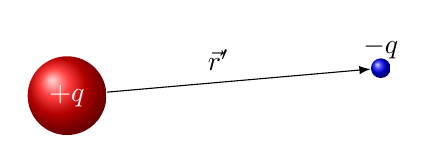
\begin{tikzpicture}
				\node[circle, inner sep=0pt, minimum  size=1cm, ball color=red, text=white] (+q) at (0,0) {$ +q $};
				\node[circle, inner sep=0pt, minimum  size=0.25cm, ball color=blue, text=white] (-q) at (5:4) {};
				\node[above] at (-q) {$ -q $};
				\draw[-latex] (+q) -- node[anchor=south east] {$ \vect{r}' $} (-q);
			\end{tikzpicture}
		\end{block}
	\end{overprint}

	\medskip

	Дипольний момент цієї системи і його друга похідна по часу
	\begin{equation*}
		\vect{p} = -q\vect{r}', \quad \ddot{\vect{p}} = -q\dot{\vect{v}},
	\end{equation*}
	де $ v =  \dot{\vect{r}}'  $ --- швидкість заряду, а $ \dot{\vect{v}} $ --- його прискорення.

	Потужність, що випромінюється:
	\begin{equation*}
		\frac{d W}{dt}  = \frac{2q^2}{3c^3}\dot{\vect{v}}^2
	\end{equation*}

	\begin{alertblock}{}
		Таким чином, електричний заряд випромінює електромагнітну
		енергію, якщо він рухається прискорено.
	\end{alertblock}
\end{frame}
% ===========================================================================




% ============================== Слайд ## ===================================
\begin{frame}[t]{Приклади}{}
	\begin{overprint}\scriptsize
		\onslide<1>
		\begin{block}{}\justifying
			Електромагнітна хвиля, що випромінюється диполем, поширюється у вакуумі так, що у хвильовій зоні на промені, перпендикулярному до осі диполя, на відстані $ r $ від нього середнє значення густини потоку енергії дорівнює $ \left\langle S \right\rangle $. Знайти середню потужність випромінювання диполя.
		\end{block}
		\onslide<2>
		\begin{block}{}\justifying
			Постійний за модулем електричний диполь моментом $ \vect{p} $ обертають з кутовою швидкістю $ \omega $ навколо осі, що перпендикулярна до осі диполя та проходить через його середину. Знайти потужність випромінювання диполя.
		\end{block}
		\onslide<3>
		\begin{block}{}\justifying
			Знайти потужність випромінювання нерелятивістської
			частинки з зарядом $ e $ і масою $ m $, що рухається круговою орбітою радіуса $ R $ у полі нерухомого точкового заряду $ q $.
		\end{block}
	\end{overprint}
\end{frame}
% ===========================================================================


\end{document}
